\section{Experimentation and results}\label{experimentations}
We detail and analyze in the section the results of the experimentation we performed using the six ML algorithms presented in Section \ref{ml_algorithms} over the two real datasets described in Section \ref{datasets}. We start by presenting our experimentation setting.

% experimentation setting
\subsection{Experimentation Setting}
All the performed tests have been done in the same machine and the same operating system. To test the performance of our six chosen ML algorithms, 
we relied on their Python implementations available through the scikit-learn library\footnote{https://scikit-learn.org/stable/}. Scikit-learn is an open source simple and efficient tool for predictive data analysis that implements
most of the existing ML algorithms. We set the following  values for the various parameters of each algorithm.
\begin{itemize}
    \item NB
    \begin{itemize}
        \item priors=None, var smoothing=1e-09.
    \end{itemize}
    \item LR
    \begin{itemize}
        \item C=1.0, class weight=None, dual=False, multi class='warn', fit intercept=True,
intercept scaling=1, 
l1 ratio=None, 
max iter=1000,                  
penalty='l2',                  
random state=0, 
solver='lbfgs', 
verbose=0,                
warm start=False,
n jobs=None,
tol=0.0001.
    \end{itemize}
    \item DT
    \begin{itemize}
        \item class weight=None, 
criterion='gini', 
max depth=None,                      
max features=None, 
max leaf nodes=None,
min samples split=2,                       
min weight fraction leaf=0.0, 
presort=False,
min impurity decrease=0.0, 
min impurity split=None,
min samples leaf=1.
    \end{itemize}
    \item RF
    \begin{itemize}
        \item  class weight=None1
criterion='gini', 
max depth=None,
max features=None, 
max leaf nodes=None,                      
min impurity decrease=0.0, 
min impurity split=None                       
min samples leaf=1,
in samples split=2,                      
min weight fraction leaf=0.0,
presort=False,
random state=0, splitter='best'.
    \end{itemize}
    \item SVM
        \begin{itemize}
        \item C=1.0, 
cache size=200,
class weight=None, 
coef0=0.0,
decision function shape='ovr', 
degree=3, 
gamma='auto', 
kernel='rbf',
max iter=-1, 
probability=True, 
random state=None, 
shrinking=True, 
tol=0.001,
verbose=False.

    \end{itemize}
    \item ANN
    \begin{itemize}
        \item activation='relu'
alpha=0.0001,
batch size='auto', 
beta1=0.9,
beta2=0.999, 
early stopping=False, 
epsilon=1e-08,
hidden layer sizes=(15, 15, 15), 
learning rate='constant',
learning rate init=0.001,
max iter=10000, momentum=0.9,
numb iter no change=10, 
nesterovs momentum=True,
power t=0.5,
random state=None,
shuffle=True, 
solver='adam', 
tol=0.0001,
validation fraction=0.1, 
verbose=False,
warm start=False.
    \end{itemize}
\end{itemize}
For the details about the description of each parameter we refer to the official documentation of the implementation of these algorithms in scikit-learn\footnote{https://scikit-learn.org/stable/supervised\_learning.html\#supervised-learning}. Concerning the segmentation of both datasets for the 
training of our ML algorithms and their testing we have considered the following splitting of the initial data.
\begin{itemize}
    \item DT1
    \begin{itemize}
        \item Training set : 70\%
        \item Test set : 30\%
    \end{itemize}
    \item DT2
    \begin{itemize}
        \item Training set : 80\%
        \item Test set : 20\%
    \end{itemize}
\end{itemize}

% performance measures 
\subsection{Performance measures}
To evaluate the performance of every classifier tested during this study, we leverage several different standard measures. We present next the definition of these performance measures.

\textbf{Precision.} 
The precision $p$, or positive value rate, for a class is the number
 of true positives (i.e. the number of cases  correctly labeled as belonging to the positive class)
 divided by the total number of cases labeled as belonging to the positive class (i.e. the sum of true positives 
and false positives, which are cases  incorrectly labeled as belonging to the class).

\textbf{ Recall.}
The recall $r$ (also known as sensitivity) is defined as the number of true positives divided by the total number of cases that actually belong
 to the positive class (i.e. the sum of true positives and false negatives, which are cases which were not labeled as belonging to the positive class but should have been).


\subsubsection*{\bf F-measure.} The F-measure, denoted by F$_1$, is a metric that measures the accuracy of a test in statistical analysis of a binary classification.
It is computed using both the precision $p$ and the recall $r$ of the test as the ratio of the number of correct positive results and the
number of all positive results returned by the classifier. 


\textbf{ Specificity.} 
The specificity, also known as the true negative rate, measures the proportion of actual negatives that are correctly identified as such 
(e.g., the percentage of people not suffering from Malaria  who are correctly identified as not having the condition).

\textbf{ Receiver operating characteristic.} A receiver operating characteristic, or ROC in short, is a graph
 that shows the diagnostic ability of a binary classifier system as its discrimination threshold is varied.
The ROC curve is created by plotting the \emph{true positive rate} (i.e. sensitivity or recall in Machine Learning) 
against the false positive rate (1 - specificity) at various threshold settings. 
The Area Under the Curve (AUC) of the ROC curve is a discrimination measure which tells us how well our predictor can classify patients in two groups: those with and those without the outcome of interest.

% Results of the experiments
\subsection{Results of the experiments}
This section presents the results of the experimentation on each real dataset for each of the six classifiers. 


\subsubsection*{\bf Experiments with DT1.}
Table  \ref{perf-measure-dt1} and Figure \ref{curve_roc_dt1} respectively show the performance measures (Precision, Recall and F-measure) and the ROC curves of the results  of our six classifiers after experimentation on the  dataset DT1. Observation shows that all classifiers have the same precision 99\% but present different recall and F-measure (see Table \ref{perf-measure-dt1}). At the same time, we note that the surfaces under the ROC curves, i.e. the AUC (Area Under the Surface) values, of the different algorithms are clearly different with values between 0.50 and 0.87.
\begin{table}[!ht]
\centering
\begin{tabular}{*{6}{c}l r}
  \toprule
  \textbf{ML algorithm} & \textbf{Precision} & \textbf{Recall} & \textbf{F1-score} \\
   \midrule
  NB &0.99& 0.17  & 0.29 \\
  LR & 0.99 & 0.92  & 0.96\\
  DT &0.99 & 0.17&0.29\\
   RF &0.99 &0.98 &0.99\\
    SVM(kernel=gaussian) &0.99 &0.98 &0.99\\
    SVM(kernel=polynom) & 0.99&0.92&0.95\\
    ANN(MLP)&0.99&0.99&0.99\\
    \bottomrule
\end{tabular}
\caption{Precision, Recall and F1-score measures over DT1}\label{perf-measure-dt1}
\end{table}

\begin{figure}[!ht]
\centering
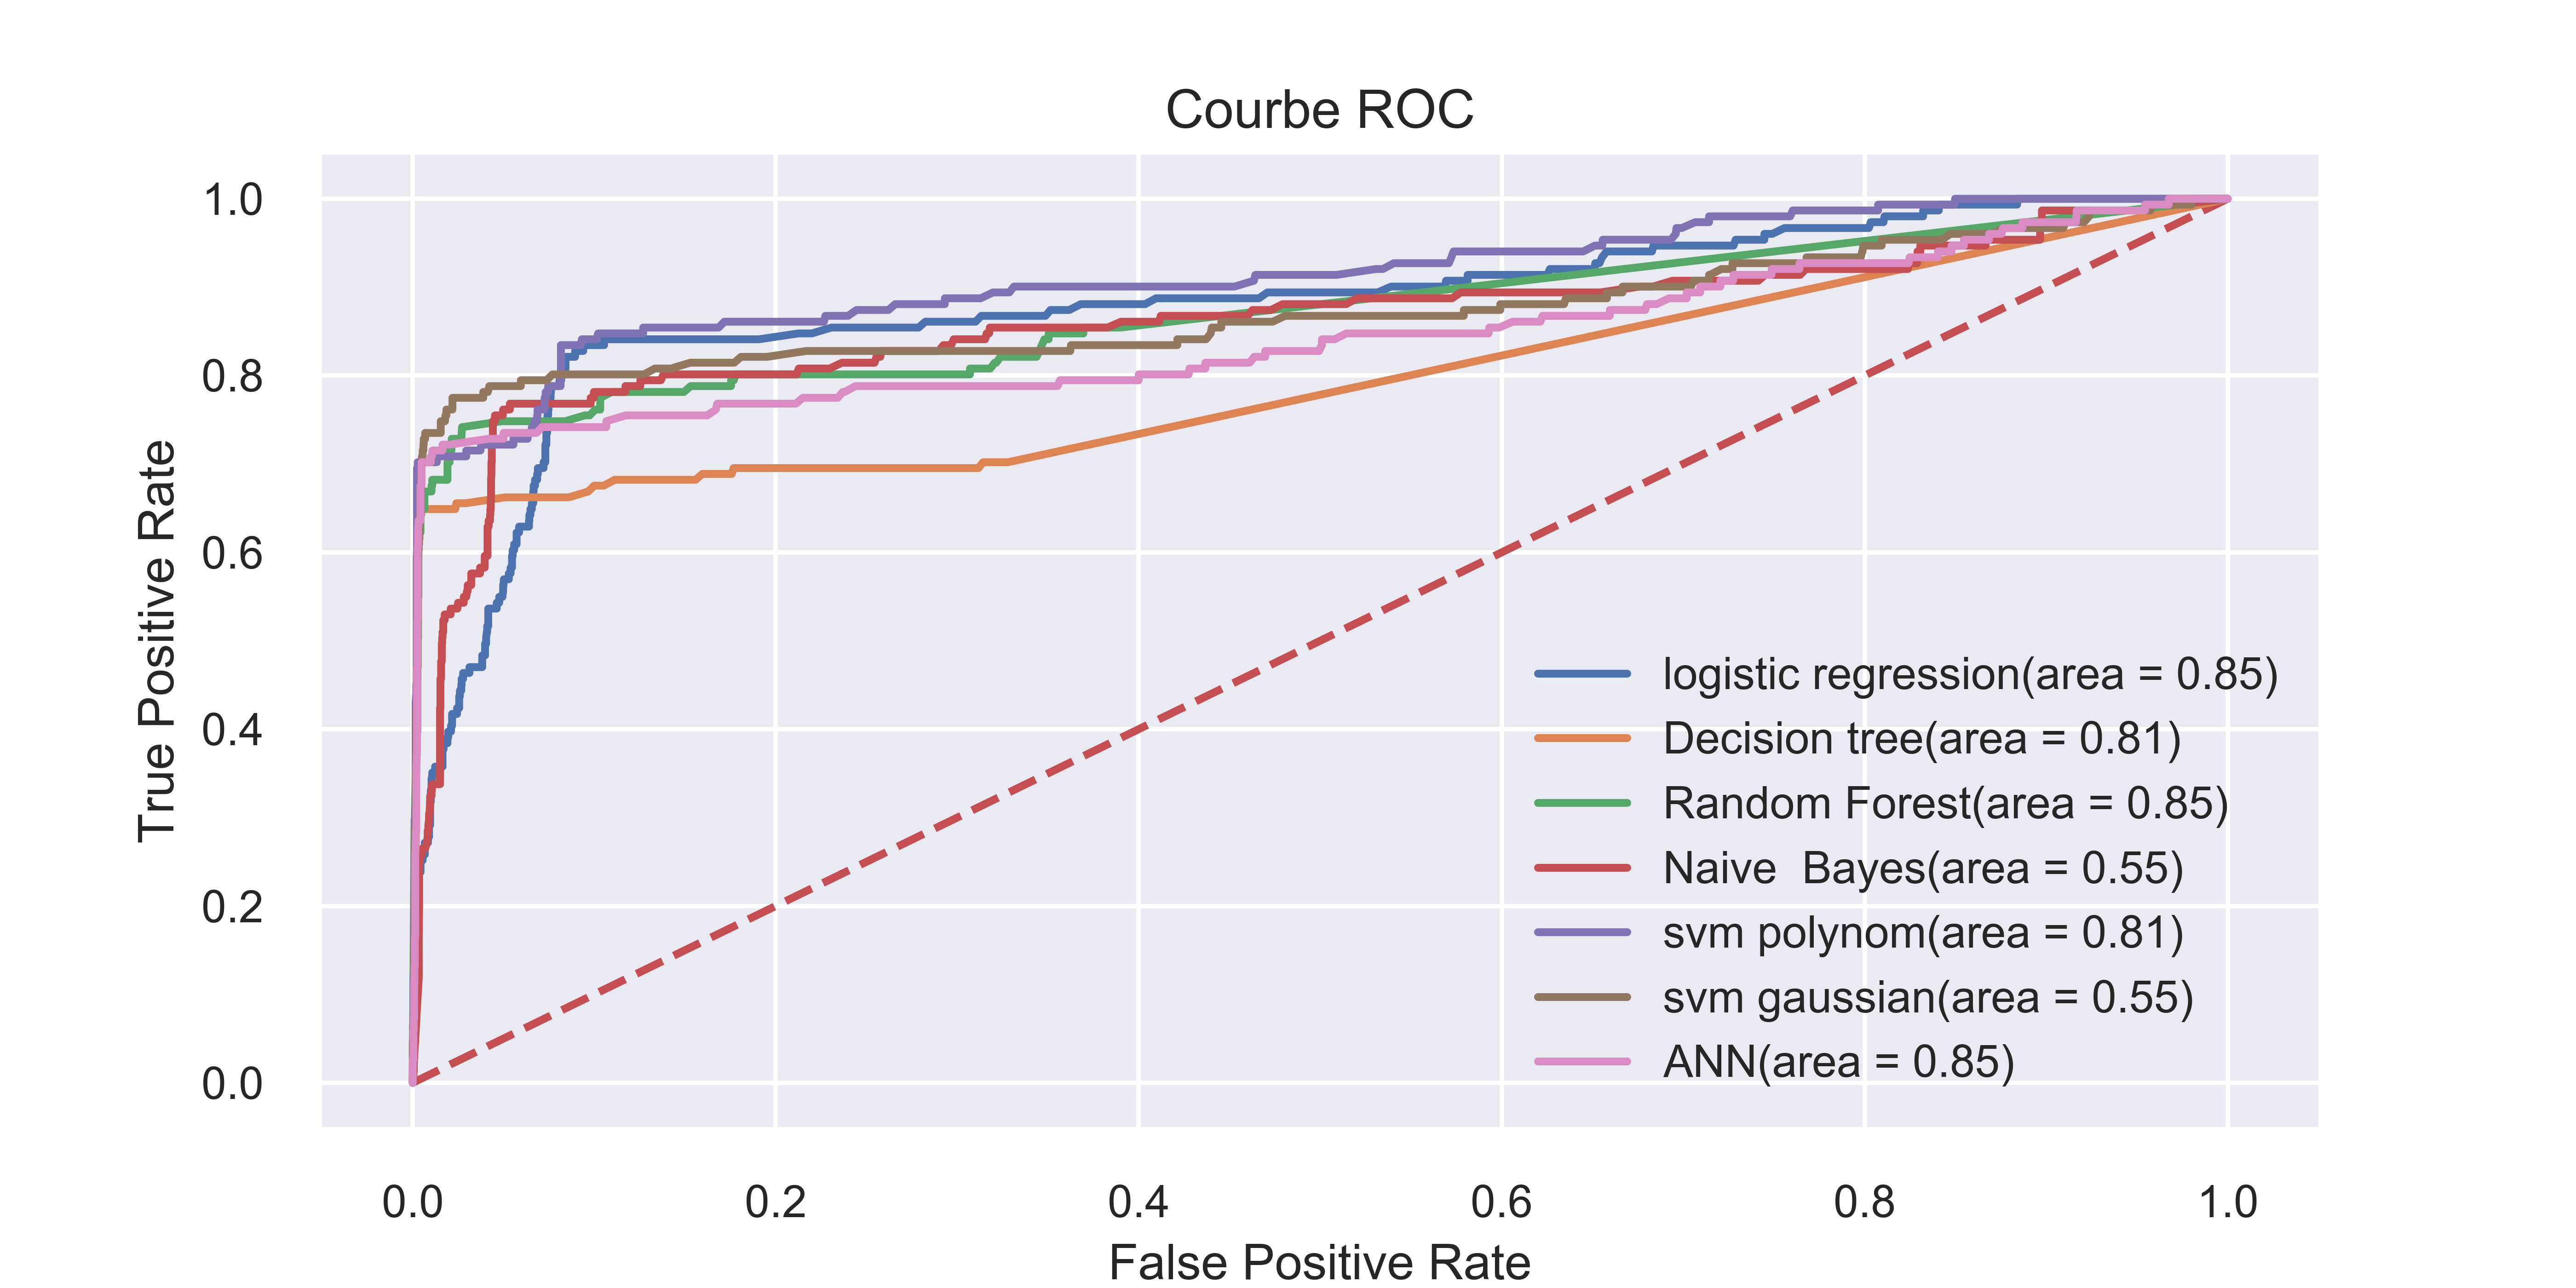
\includegraphics[width=.5\textwidth]{ROCmg}
\caption{True Positive Rate over False Positive Rate on DT1}\label{curve_roc_dt1}
\end{figure}

\subsubsection*{\bf Experiments with DT2.}
Table \ref{perf-measure-dt2} and Figure \ref{curve_roc_dt2} respectively show the performance measures (Precision, Recall and F-measure) and the ROC curves of our six classifiers after experimentation on the dataset DT2. In contrast to the results obtained with DT1, we notice that our classifiers have overall precision which are slightly down and vary between 93\% and 96\% (see Table \ref{perf-measure-dt2}). Likewise ROC curves follow the same trends with AUC values between 0.50 and 0.70

\begin{table}[!ht]
\centering
\begin{tabular}{*{5}{c}l r}
  \toprule
  \textbf{ML algorithm} & \textbf{Precision} & \textbf{Recall} & \textbf{F1-score} \\
   \midrule
  NB &0.96& 0.05  & 0.10 \\
  LR & 0.93& 0.62  & 0.75\\
  DT &0.92 & 0.85&0.88\\
   RF &0.92 &0.85&0.89\\
    SVM(kernel=gaussian) &0.92 &0.86 &0.89\\
    SVM(kernel=polynom) & 0.93&0.54&0.68\\
    ANN(MLP)&0.93&0.85&0.89\\
    \bottomrule
\end{tabular}
\caption{Precision, Recall and F1-score measures on DT2}\label{perf-measure-dt2}
\end{table}
\begin{figure}[!h]
\centering
%\subfigure[Prediction whith DT2]{
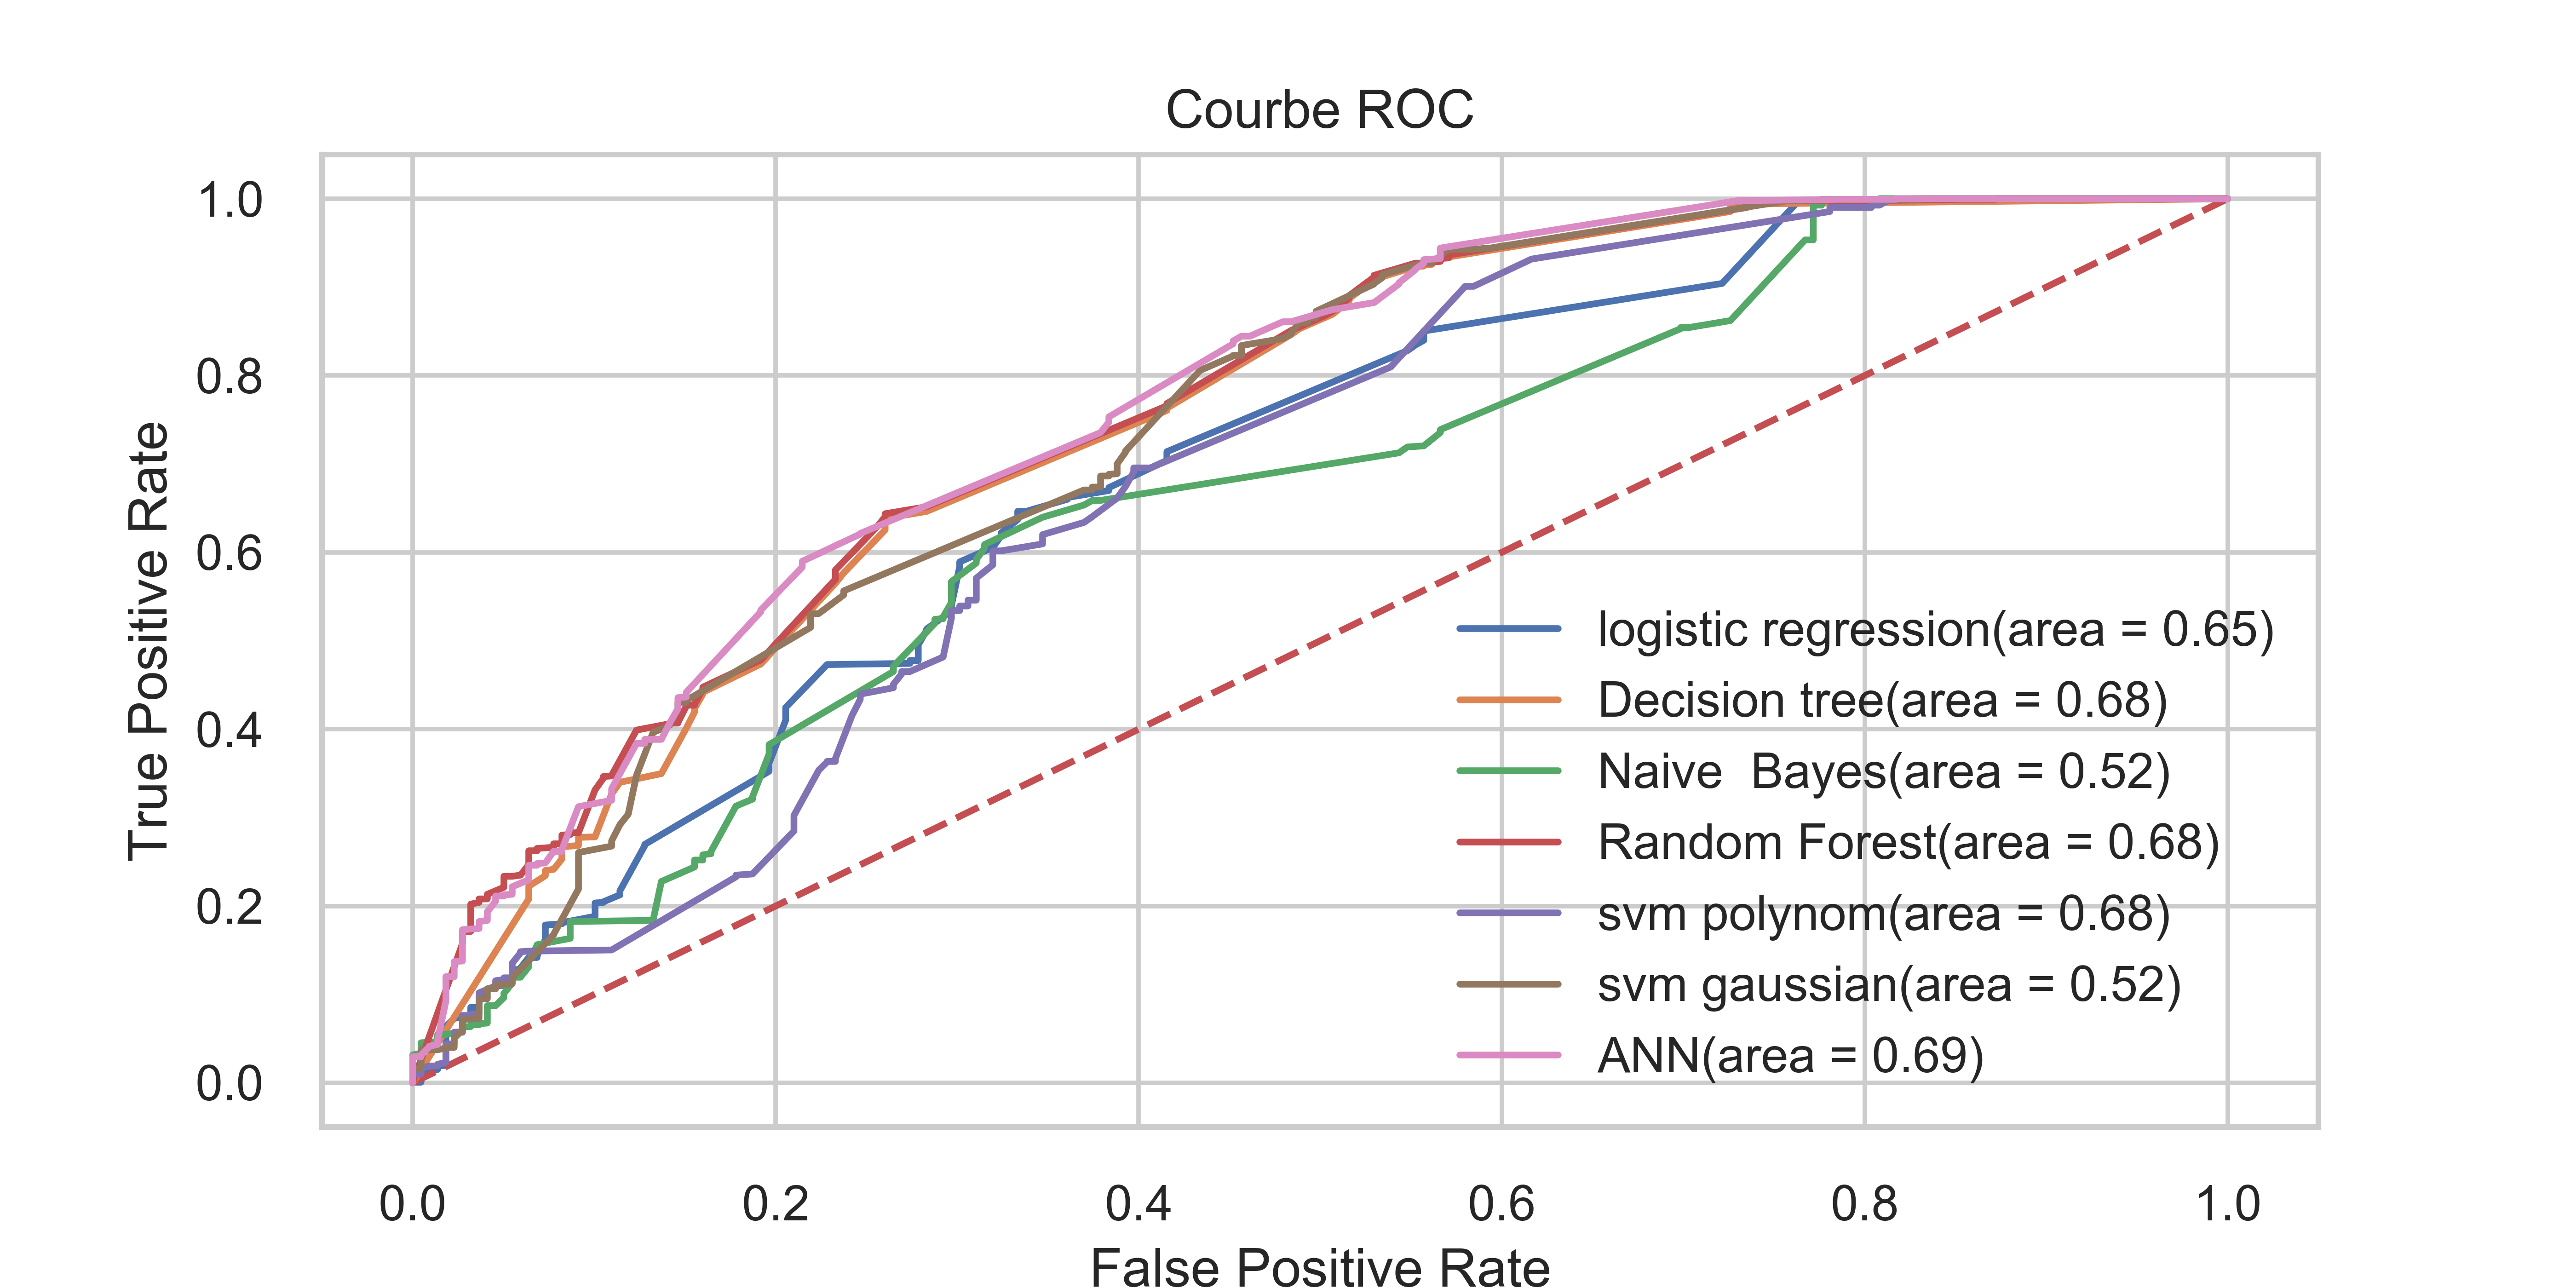
\includegraphics[width=0.5\textwidth]{ROCdio}
%}
\caption{True Positive Rate over False Positive Rate on DT2}\label{curve_roc_dt2}
\end{figure}
\subsection{Analysis of the results and discussion}

\begin{figure}[!ht]
\begin{tikzpicture}
\begin{axis}
[
xlabel = Tree depth,
ylabel = Accuracy of DT (\%)
]
\addplot[mark=halfcircle, only marks] table [x=height, y=accu] {accu_tree_height.csv};
\end{axis}
\end{tikzpicture}
\caption{Accuracy of DT  with respect to the tree depth}\label{accy_dt_tree_height}
\end{figure}
%
%
\begin{figure}[!ht]
\begin{tikzpicture}
\begin{axis}
[
xlabel = Number of estimators,
ylabel = Accuracy of RF (\%)
]
\addplot[color=red, mark=halfcircle, only marks] table [x=nb_estimator, y=accu] {accu_estimators_rf.csv};
\end{axis}
\end{tikzpicture}
\caption{Accuracy of RF  with respect to the number of used decision trees}\label{accu_RF_n_trees}
\end{figure}
%
\begin{figure}[!ht]
\begin{tikzpicture}
\begin{axis}
[
xlabel = Number of hidden layers,
ylabel = Accuracy of ANN (\%)
]
\addplot[color=blue, mark=halfcircle, only marks] table [x=nb_layers, y=accu] {accu_ann_hidden_layers.csv};
\end{axis}
\end{tikzpicture}
\caption{Accuracy of ANN with respect to the number of hidden layers}\label{accu_ann_hidden_layers}
\end{figure}

Analyzing in details the performance of our six classifiers on both datasets, the results of the previous section clearly argue in favor of the classifiers RF, LR, SVM with Gaussian kernel and ANN. Indeed considering the datase DT1, that contains observations about patients living in different areas in Senegal, these four classifiers have a precision of 99\%, a recall above 92\% and a F-measure above 95\%. We note the same trend with the dataset DT2 which contains observations about patients living in the same area in Senegal.  So in terms of precision, recall and F-measure those four classifiers outperform the rest. We can also remark that RF, LR, SVM with Gaussian kernel, and ANN present better precision than the systematically performed and used Rapid Diagnostic Test within the majority of health structures in Senegal.
The difference of performance of our classifiers on the two datasets  can be explained by the fact that climatic factors such as temperature and standing water are very determining in the appearance or not of Malaria in distinct areas in Senegal as they favor the development of mosquitoes responsible for the disease.

When we now restrict ourselves to the ROC curves, we observe that SVM with Gaussian kernel and Naive Bayes present the worst positive prediction rate as they have the lowest AUC values compared to the other classifiers.

In addition we have tried to study the impact of the tree depth, the number of hidden layers and the number of estimators for DT, ANN and RF respectively. While the increase of the tree depth decreases the accuracy of DT (see Figure  \ref{accy_dt_tree_height}), the highest accuracy of RF corresponds to the use of 50 estimators as shown in Figure \ref{accu_RF_n_trees}. Furthermore, Figure \ref{accu_ann_hidden_layers} shows that when the number of hidden layers increases the accuracy of ANN does so in general.
To conclude, we can argue that ANN seems to be the most promising classification approach among the six studied ML algorithms when we are only interested by the precision, recall and F-measure. If we include the ROC curves in the analysis ANN remains the most efficient approach.

